\documentclass{mwart}
\usepackage{multicol}
\usepackage{polski} % Pozwala na użycie polskiego. Ustawia między innymi fontenc na T1
\usepackage[utf8]{inputenc} % Informuje o kodowaniu
\usepackage{enumitem}
\usepackage{xcolor}
\usepackage{xcolor}% http://ctan.org/pkg/xcolor
\usepackage{hyperref}
\usepackage{listings}
\usepackage{float} % Ustawianie obrazów
\usepackage[caption = false]{subfig} % Wiele obrazów w jednej figurze
\definecolor{LinkColor}{HTML}{1d5cc1}
\renewcommand{\labelitemi}{\textbullet} % Zmiana symbolu wliczeń

\lstset{
  basicstyle=\ttfamily,
  columns=fullflexible,
  breaklines=true,
  postbreak=\mbox{\textcolor{red}{$\hookrightarrow$}\space},
}

\definecolor{LinkColor}{HTML}{1d5cc1}

\usepackage{tabto}

\usepackage{graphicx} % Pakiet do obrazów
\graphicspath{ {./Obrazy/} } % Folder, z którego będą brane obrazy

% Nie twórz nowych stron
\usepackage{etoolbox}
\makeatletter
% \patchcmd{\chapter}{\if@openright\cleardoublepage\else\clearpage\fi}{}{}{}
\makeatother

\title{Raport końcowy -- Gra w życie}
\author{Krzysztof Dąbrowski i Jakub Bogusz}
\date{\today}

\begin{document}
\maketitle{}

\tableofcontents{}

\section{Ostateczny projekt modułów}
\paragraph{Zmodyfikowany diagram modułów:}\mbox{}\\
\begin{figure}[H]
	\centering
	\def\svgwidth{\columnwidth}
	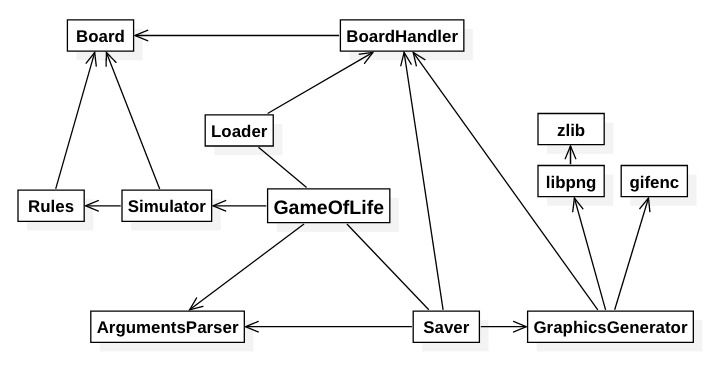
\includegraphics[width=13cm]{diagram_modulow.png}
\end{figure}

\section{Opis modyfikacji}
W trakcie pracy nad projektem okazało się, że niektóre problemy można rozwiązać lepiej niż przewiduje to specyfikacja impleilementacyja. Pojawiły się również nieprzewidziane problemy z wyświetlaniem bardzo małych obrazów przez typowe programy do prezentacji grafik. Z tych powodów wprowadzone zostały pewne zmiany.

\subsection{GameOfLife}
Specyfikacja nie przewidywał funkcji odpowiedzialnej z główny przebieg sterowania w programie. Dodano więc funkcję \texttt{void runProgram(int argc, char **args)}.
Koordynuje ona pracę wszystkich pozostałych modułów.

\subsection{ArgumentsParser}
Do typu wyliczeniowego \texttt{FileType} (dawniej \texttt{Type}) została dodana nowa wartość ,,OUT'' reprezentująca wypisywanie kolejnych stanów na standartowe wyjście.

Do struktury \texttt{Config} zostały dodane nowe pola \texttt{sizeX} i \texttt{sizeY} reprezentujące wymiary planszy. 

Dodano funkcję \texttt{void disposeConfig(Config *config)}, która zwalnia pamięć zarezerwowaną na tą strukturę.

\subsection{BoardSaver}
Nazwa modułu została zmieniona na \texttt{Saver}, a jego struktura gruntownie zmodyfikowana.

Aktualna postać modułu:\\
\texttt{void saveAsPng(Board** history, Config* config, int i)} -- Zapis kolejnych pokoleń do plików png.
\begin{itemize}[label={}]
	\item\texttt{Board** history} -- tablica wskaźników na struktury reprezentujące kolejne pokolenia,
	\item\texttt{Config* config} -- wskaźnik na strukturę ustawień generacji kolejnych pokoleń,
	\item \texttt{int i} -- numer aktualnie generowanego pokolenia. Potrzebny do generowania nazw plików.
\end{itemize}

\noindent{}\texttt{void saveAsGif(Board** history, Config* config, int historySize)} -- Zapis kolejnych pokoleń do pliku gif.
\begin{itemize}[label={}]
	\item\texttt{Board** history} -- tablica wskaźników na struktury reprezentujące kolejne pokolenia,
	\item\texttt{Config* config} -- wskaźnik na strukturę ustawień generacji kolejnych pokoleń,
	\item \texttt{int historySize} -- Liczba pokoleń w historii
\end{itemize}

\noindent{}\texttt{void saveAsTxt(Board** history, Config* config, int i)} -- Zapis kolejnych pokoleń do plików txt.
\begin{itemize}[label={}]
	\item\texttt{Board** history} -- tablica wskaźników na struktury reprezentujące kolejne pokolenia,
	\item\texttt{Config* config} -- wskaźnik na strukturę ustawień generacji kolejnych pokoleń,
	\item \texttt{int i} -- numer aktualnie generowanego pokolenia. Potrzebny do generowania nazw plików.
\end{itemize}

\noindent{}\texttt{void printToStdout(Board** history, Config* config, int i)} -- Wyświetlenie kolejnych pokoleń w terminalu.
\begin{itemize}[label={}]
	\item\texttt{Board** history} -- tablica wskaźników na struktury reprezentujące kolejne pokolenia,
	\item\texttt{Config* config} -- wskaźnik na strukturę ustawień generacji kolejnych pokoleń,
	\item \texttt{int i} -- numer aktualnie generowanego pokolenia. Potrzebny do generowania nazw plików.
\end{itemize}

\subsection{GraphicsGenerator}
W tym module zostały dodane nowe funkcje pomocnicze związane z przeskalowywaniem obrazu. Okazało się, że po stworzeniu obrazu, o rozmiarze w pikselach takich jak plansza, domyślnie jest on wyświetlany w bardzo małej wielkości przez typowe programy. By tego uniknąć dodana została funkcjonalność przeskalowywania obrazów do minimalnej wielkości.

By skalowanie było uniwersalne pracuje ono na wartościach pikseli, z których ma powstać grafika. Dzięki temu jest niezależne od palet barw, które są różne dla generowania png i gif. Do przechowywania wartości pikseli używany jest nowy typ \texttt{Pixel}.

Skalowanie może tylko zwiększyć wymiary obrazu.

\subsubsection{Nowe funkcje}
Na potrzeby skalowania zostały napisane następujące funkcje:\\
\noindent{}\texttt{Pixel *translateBoardToPixels(Board *board, Pixel valueOfAlive, Pixel valueOfDead)} -- Zamiana planszy na tablicę pikseli.
\begin{itemize}[label={}]
	\item\texttt{Board *board} -- wskaźnik na planszę, która ma być przedstawiona jako piksele,
	\item\texttt{Pixel valueOfAlive} -- wartość pikseli dla żywych komórek,
	\item \texttt{Pixel valueOfDead} -- wartość pikseli dla martwych komórek.
\end{itemize}
Zwracany jest wskaźnik na dynamicznie przydzieloną tablicę pikseli odpowiadającą otrzymanej planszy.\\

\noindent{}\texttt{void getUpscaledImageSize(int orginalX, int orginalY, int *newX, int *newY)} -- Obliczenie wymiarów obrazu po przeskalowaniu.
\begin{itemize}[label={}]
	\item\texttt{int orginalX} -- szerokość oryginalnego obrazu,
	\item\texttt{int orginalY} -- wysykość oryginalnego obrazu,
	\item \texttt{int *newX} -- wskaźnik na zmienną typu int, gdzie zostanie zapisana nowa szerokość planszy,
	\item \texttt{int *newY} -- wskaźnik na zmienną typu int, gdzie zostanie zapisana nowa wysokość planszy.
\end{itemize}

\noindent{}\texttt{Pixel *upscaleImage(const Pixel *original, int imageX, int imageY)} -- Przeskalowanie obrazu.
\begin{itemize}[label={}]
	\item\texttt{const Pixel *original} -- wskaźnik na tablicę pikseli reprezentującą oryginalny obraz,
	\item\texttt{int imageX} -- szerokość oryginalnego obrazu,
	\item \texttt{int imageY} -- wysokość oryginalnego obrazu,
\end{itemize}
Zwracany jest wskaźnik na dynamicznie przydzieloną tablicę pikseli odpowiadającą przeskalowanemu obrazowi.

\subsubsection{Zmiany już istniejących funkcji}
Funkcja \texttt{savePng} nie przyjmuje ustawień \texttt{Config* c}. Nie są one potrzebne do generowania obrazu. Zamiast tego przyjmuję nazwę pliku jaki ma być generowany. Dodatkowo zamiast tekstu \texttt{char* data} jako pierwszy argument przyjmuje strukturę planszy. Dzięki temu została wyeliminowana zbędna serializacja i parsowanie planszy.

Nazwa funkcji \texttt{saveGif} została zmieniona na \texttt{saveHistoryAsGif} ponieważ w bibliotece do towrzenia gifów istniej już funkcja o takiej nazwie. Funkcja ta również zamiast struktury ustawień otrzymuje nazwę pliku, który ma zostać wygenerowany.

\section{Prezentacja działania}
Przykłady wywołania programu z różnymi flagami.

\subsection{Generacja obrazów z wczytaniem stanu z pliku}
\noindent{}Wywołanie programu: \\
\texttt{./game-of-life -f input.txt -t png -o raport -n 6} \\
Argumenty:
\begin{itemize}
\item \texttt{-f input.txt} -- Stan początkowy jest wczytany z pliku ,,input.txt'',
\item \texttt{-t png} -- Zostanie wygenerowana seria plików .png z kolejnymi pokoleniami,
\item \texttt{-o raport} -- Wygenerowane pliki zostaną zapisane do podfolderu w folderze ,,raport'',
\item \texttt{-n 6} -- Zostanie wygenerowanych 6 następnych pokoleń .png (ze stanem początkowym 7 obrazków).
\end{itemize}

\newpage{}
\subsubsection*{Powstałe obrazy}
Program wygenerował poniższe pliki. Przedstawiają ruch struktury szybowca.

\begin{figure}[H]
  \setlength{\fboxsep}{0pt} %Wielkości ramek
  \setlength{\fboxrule}{1pt}

  \centering
  \subfloat[Pokolenie 0]{\fbox{
\includegraphics[width = 5cm]{glider0}}}
  \hspace{0.7cm}
  \subfloat[Pokolenie 1]{\fbox{
\includegraphics[width = 5cm]{glider1}}}\\
  \subfloat[Pokolenie 2]{\fbox{
\includegraphics[width = 5cm]{glider2}}}
  \hspace{0.7cm}
  \subfloat[Pokolenie 3]{\fbox{
\includegraphics[width = 5cm]{glider3}}}\\
  \subfloat[Pokolenie 4]{\fbox{
\includegraphics[width = 5cm]{glider4}}}
  \hspace{0.7cm}
  \subfloat[Pokolenie 5]{\fbox{
\includegraphics[width = 5cm]{glider5}}} 
  
  \caption{Wygenerowane pliki}
  \label{fig:GliderExample}
\end{figure}



\subsection{Generacja plików tekstowych  z wczytaniem losową planszą początkową}
\noindent{}Wywołanie programu: \\
\texttt{./game-of-life -s 5x5 -t txt -o raport -n 10} \\
Argumenty:
\begin{itemize}
\item \texttt{-s 5x5} -- Zostanie wygenerowana losowa plansza początkowa w rozmiarach 5 na 5 komórek,
\item \texttt{-t txt} -- Zostanie wygenerowana seria plików .txt z kolejnymi pokoleniami,
\item \texttt{-o raport} -- Wygenerowane pliki zostaną zapisane do podfolderu w folderze ,,raport'',
\item \texttt{-n 3} -- Zostanie wygenerowanych 3 następnych pokoleń .png (ze stanem początkowym 4 plików tekstowych).
\vspace{5mm}
\end{itemize}
\begin{center}
\begin{multicols}{2}
[\textbf{Wygenerował pliki o poniższej zawartości:}]
\texttt{
\\\hspace{-13mm}5 5\\
1 1 1 1 1\\
0 0 1 1 0\\
1 0 1 1 1\\
1 1 0 1 0\\
1 1 0 0 1\\
}
Jako pokolenie początkowe.\\
\texttt{
\\\hspace{-13mm}5 5\\
0 1 0 0 1\\
1 0 0 0 0\\
1 0 0 0 1\\
0 0 0 0 0\\
1 1 1 0 0\\
}
Jako pokolenie pierwsze.\\
\texttt{
\\\hspace{-13mm}5 5\\
0 0 0 0 0\\
1 1 0 0 0\\
0 0 0 0 0\\
1 0 0 0 0\\
0 1 0 0 0\\
}
Jako pokolenie drugie.\\
\texttt{
\\\hspace{-13mm}5 5\\
0 0 0 0 0\\
0 0 0 0 0\\
1 1 0 0 0\\
0 0 0 0 0\\
0 0 0 0 0\\
}
Jako pokolenie trzecie.\\
\end{multicols}
\end{center}


\subsection{Generacja plików gif z losową planszą}
\noindent{}Wywołanie programu: \\
\texttt{./game-of-life -s 20x20 -o raport -n 50} \\
Argumenty:
\begin{itemize}
\item \texttt{-s 20x20} -- Zostanie wygenerowana losowa plansza początkowa w rozmiarach 20 na 20 komórek,
\item \texttt{-o raport} -- Wygenerowany plik zostanie zapisany z folderze raport,
\item \texttt{-n 50} -- Zostanie wygenerowanych 50 następnych pokoleń w formie jednego pliku .gif (ze stanem początkowym 51 klatek).\\
\end{itemize}
Nie podanie formatu pliku wynikowego spowoduje wygenerowanie pliku .gif.
\vspace{5mm}
Wyniki pracy programu dostępne \href{https://github.com/SiwyKrzysiek/gra-w-zycie/tree/report/code/raport}{\textcolor{LinkColor}{pod linkiem}}.

\subsection{Wyświetlenie kolejnych pokoleń w konsoli z planszą pobieraną z pliku}
\noindent{}Wywołanie programu: \\
\texttt{./game-of-life -f input.txt -t out -n 20 -d 500} \\
Argumenty:
\begin{itemize}
\item \texttt{-f input.txt} -- Stan początkowy jest wczytany z pliku ,,input.txt'',
\item \texttt{-t out} -- kolejne pokolenia zostaną wyświetlone na konsoli,
\item \texttt{-n 50} -- Zostanie wygenerowanych 50 następnych pokoleń w formie jednego pliku .gif (ze stanem początkowym 51 klatek),
\item \texttt{-d 500} -- Kolejne pokolenia będą wyświetlane co 500ms.\\
\end{itemize}

\noindent Takie wywołanie programu wyświetli kolejne pokolenia w terminalu zachowując pół sekundowe odstępy między kolejnymi stanami planszy w formacie podobnym do wyników z plików tekstowych (bez wymiarów planszy).

\section{Podsumowanie testów modułów}
Do pisania oraz automatyzacji wykonania testów jednostkowych został wykorzystany framework \textit{CUnit}. Dzięki temu na dowolnym etapie projektu można było łatwo sprawdzić poprawność już istniejącego kodu.

\subsection{Wygenerowany raport}
Wyniki testów jednostkowych przedstawia poniższy raport.

\begin{verbatim}

  CUnit - A unit testing framework for C - Version 2.1-3
  http://cunit.sourceforge.net/


Suite: Board tests
Test: To string test ...passed
Suite: Loader tests
Test: Parse small file test ...passed
Suite: Rules tests
Test: Dead cell stays dead ...passed
Test: Dead cell comes to live ...passed
Test: Alive cell dies from overpopulation ...passed
Test: Alive cell dies from loneliness ...passed
Test: Alive cell stays alive ...passed
Suite: Simulator tests
Test: Simulate one next generation on small board ...passed

Run Summary:    Type  Total    Ran Passed Failed Inactive
           suites      4      4    n/a      0        0
            tests      8      8      8      0        0
          asserts     27     27     27      0      n/a

Elapsed time =    0.001 seconds
\end{verbatim}

\subsection{Wnioski}
Z raportu testów jednostkowych wynika, że wszystkie wszystkie sprawdzane funkcjonalności dają prawidłowe wyniki. Wszystkie testy są oznaczone jako \texttt{...passed} oraz liczba zapewnień, których wyniki są poprawne jest równa liczbie wszystkich zapewnień.


\section{Analiza pamięci}
\noindent Raport programu \texttt{valgrind } zwraca następujące wyniki:\\\\
\noindent \texttt{\noindent 
==18728== LEAK SUMMARY:\\
==18728==    definitely lost: 0 bytes in 0 blocks\\
==18728==    indirectly lost: 0 bytes in 0 blocks\\
==18728==      possibly lost: 72 bytes in 3 blocks\\
==18728==    still reachable: 23,728 bytes in 28 blocks\\
==18728==         suppressed: 18,077 bytes in 153 blocks\\
\\
==18728== ERROR SUMMARY: 0 errors from 0 contexts 
}\\\\

2 pierwsze linie raportu informują o braku definitywnych wycieków pamięci, co oznacza że program prawidłowo zarządza pamięcią.

Wycieki oznaczone jako \texttt{still reachable} oraz \texttt{possibly lost} spowodowane są przez funkcje bibliotek \texttt{ctime} oraz \texttt{libpng}, więc nie mamy na nie wpływu i nie jesteśmy w stanie ich wyeliminować. Załączamy fragmentu raportu opisujące te wycieki:\\

\paragraph{possible leaks:} \mbox{}

\begin{scriptsize}
\noindent \texttt{\noindent 
\\==18752== 72 bytes in 3 blocks are possibly lost in loss record 34 of 60
\\==18752==    at 0x1000B26EA: calloc (in /usr/local/Cellar/valgrind/3.14.0/lib/valgrind/vgpreload\_memcheck-amd64-darwin.so)
\\==18752==    by 0x1007AD7C2: map\_images\_nolock (in /usr/lib/libobjc.A.dylib)
\\==18752==    by 0x1007C04E0: map\_images (in /usr/lib/libobjc.A.dylib)
\\==18752==    by 0x10000DC64: dyld::notifyBatchPartial(dyld\_image\_states, bool, char const* (*)(dyld\_image\_states, unsigned int, dyld\_image\_info const*), bool, bool) (in /usr/lib/dyld)
\\==18752==    by 0x10000DE39: dyld::registerObjCNotifiers(void (*)(unsigned int, char const* const*, mach\_header const* const*), void (*)(char const*, mach\_header const*), void (*)(char const*, mach\_header const*)) (in /usr/lib/dyld)
\\==18752==    by 0x10027871D: \_dyld\_objc\_notify\_register (in /usr/lib/system/libdyld.dylib)
\\==18752==    by 0x1007AD073: \_objc\_init (in /usr/lib/libobjc.A.dylib)
\\==18752==    by 0x100202B34: \_os\_object\_init (in /usr/lib/system/libdispatch.dylib)
\\==18752==    by 0x100202B1B: libdispatch\_init (in /usr/lib/system/libdispatch.dylib)
\\==18752==    by 0x1001119C2: libSystem\_initializer (in /usr/lib/libSystem.B.dylib)
\\==18752==    by 0x10001FAC5: ImageLoaderMachO::doModInitFunctions(ImageLoader::LinkContext const\&) (in /usr/lib/dyld)
\\==18752==    by 0x10001FCF5: ImageLoaderMachO::doInitialization(ImageLoader::LinkContext const\&) (in /usr/lib/dyld)
}
\end{scriptsize}
\\

\paragraph{still reachable:}\mbox{}

\begin{scriptsize}
\noindent \texttt{\noindent 
\\==18805== 18,280 bytes in 1 blocks are still reachable in loss record 60 of 60
\\==18805==    at 0x1000B26EA: calloc (in /usr/local/Cellar/valgrind/3.14.0/lib/valgrind/vgpreload\_memcheck-amd64-darwin.so)
\\==18805==    by 0x100351930: tzsetwall\_basic (in /usr/lib/system/libsystem\_c.dylib)
\\==18805==    by 0x1003537C9: localtime (in /usr/lib/system/libsystem\_c.dylib)
\\==18805==    by 0x100353945: ctime (in /usr/lib/system/libsystem\_c.dylib)
\\==18805==    by 0x1000039AF: setup (Saver.c:5)
\\==18805==    by 0x100003A2E: saveCommon (Saver.c:12)
\\==18805==    by 0x100003E59: saveAsPng (Saver.c:53)
\\==18805==    by 0x10000405E: runProgram (main.c:83)
\\==18805==    by 0x100003F31: main (main.c:32)
}
\end{scriptsize}

\end{document}


